\documentclass[10pt,twocolumn,letterpaper]{article}

\usepackage{cvpr}
\usepackage{times}
\usepackage{epsfig}
\usepackage{graphicx}
\usepackage{amsmath}
\usepackage{amssymb}
\usepackage{booktabs}
\usepackage{multirow}

\usepackage[breaklinks=true,bookmarks=false]{hyperref}

\cvprfinalcopy

\def\cvprPaperID{****}
\def\httilde{\mbox{\tt\raisebox{-.5ex}{\symbol{126}}}}

\setcounter{page}{1}
\begin{document}

\title{Studying the Limitations of Distributed Graph Reinforcement\\
Learning for Packet Routing: An Empirical Analysis of ScaIR}

\author{Miquel Ainaud\\
{\tt\small miquel.ainaud@estudiantat.upc.edu}
\and
Josep Vidal\\
{\tt\small josep.vidal@upc.edu}
}

\maketitle

\begin{abstract}
Packet routing in large networks is a combinatorial optimisation problem
whose difficulty grows with traffic complexity. Recently, methods combining
multi-agent reinforcement learning with graph neural networks (GNNs) have
been proposed to learn congestion-aware routing policies. Among these,
ScaIR uses a per-node sub-GNN to compress topology information into a
feature vector that feeds a deep Q-network. We implement ScaIR from
scratch and evaluate it on four real backbone topologies with measured
traffic matrices. Our systematic investigation reveals that the sub-GNN
does not actually learn meaningful topology structure: replacing it with
a fixed one-hot node identifier or a static connectivity mask yields
equal or better performance within the same training budget. The GNN
feature vectors converge to encodings that are informationally
equivalent to a node identity label, making the architecture essentially
a distributed Q-network with indexed nodes. This explains two
simultaneously observed phenomena: the ablation failure
(any fixed identity encoding performs as well as the GNN) and the
topology change fragility (introducing a new node is catastrophic because
its identity is unknown to the trained model). We argue that ScaIR's
gains over OSPF come from the multi-agent DQN and UCB exploration
mechanism, not from the GNN component, and discuss what a more
principled topology encoding would require.
\end{abstract}

\section{Introduction}

Packet routing is a fundamental task in computer networking: when a router
receives a packet, it must decide to which neighbouring node to forward it
so that the packet reaches its destination with minimum delay. The dominant
deployed solution, OSPF, uses Dijkstra's algorithm to precompute the
shortest path in terms of hop count \cite{dijkstra1959}. This works well
when traffic is spread uniformly across source--destination pairs, but degrades severely under
congestion: when a large fraction of packets is concentrated on a small
number of paths, OSPF routes them all along the same shortest path,
which saturates, while alternative routes remain idle.

Reinforcement learning (RL) offers a natural framework to address this
limitation. A router trained with RL can learn to route around
congested links, trading a few extra hops for lower queuing delays. The
earliest such method, Q-routing \cite{boyan1994}, modelled each router
as an agent and used Q-learning to minimise per-hop delay. Its main
limitation is scalability: Q-tables grow with topology size, and the
Q-values of individual routers are not shared, so each agent learns only
from its local experience. Deep Q-routing \cite{mukhutdinov2019} and
subsequent systems such as DQRC \cite{you2020} and PER-D3QN
\cite{bai2024} replace Q-tables with neural networks and introduce
one-hop neighbour communication, allowing agents to share approximate
Q-values and take more globally-informed decisions.

A recurring theme in this literature is the role of graph neural networks
(GNNs). GNNs process data defined on graphs by iteratively aggregating
information from neighbours, making them a natural fit for topology-aware
feature extraction in routing. RouteNet \cite{rusek2020} uses GNNs to
predict network performance metrics from topology and traffic in a
centralised setting. ScaIR \cite{scair2025} brings this idea into the
distributed multi-agent RL framework: each router maintains its own
sub-GNN that exchanges feature vectors with its direct neighbours and
compresses the neighbourhood topology into a fixed-length representation,
which is then used as an additional input to the Q-network. The
sub-GNN is fully distributed (no global topology needed), trained
jointly with the Q-network, and is claimed to give each agent a
compressed view of the global network state.

ScaIR presents results showing meaningful advantages over OSPF and
competing RL methods, and the architecture is conceptually appealing.
In this work, we implement ScaIR from scratch and ask a critical
question: does the sub-GNN actually encode useful topology information,
or is it a complexity overhead that converges to something much simpler?
Our experiments reveal that the answer is the latter, and that this has
important consequences for the model's generalisation to topology
changes.

Our main goals are: (i) to reproduce ScaIR's performance claims on
multiple topologies; (ii) to isolate the contribution of the GNN from
the contribution of the Q-network and exploration strategy through
controlled ablations; (iii) to characterise the model's behaviour under
topology changes and traffic shifts; and (iv) to assess how close the
learned policy is to a theoretical online optimum.

\section{Architecture of ScaIR}
\label{sec:arch}

\subsection{Network model and simulation environment}

We model the network as an undirected graph $G = (N, L)$ where $N$ is
the set of routers and $L$ the set of bidirectional links. Following the
ScaIR paper, we adopt a fully distributed architecture: each router
makes forwarding decisions independently based only on its own local
observations and information received from its one-hop neighbours.
There is no centralised controller and no global topology knowledge.

Packets arrive at each source router following a Poisson process with
mean inter-arrival time $G_i = 0.5$\,ms. Source--destination pairs are
sampled proportional to a measured real-world traffic matrix $\mathbf{T}$,
with a fraction $D_r \in [0,1]$ of packets forced onto a designated
hot-spot pair to simulate congestion. The diagonal of $\mathbf{T}$ is
zeroed so that self-routing never occurs. Each router maintains a FIFO
queue per outgoing interface and processes packets sequentially. The
forwarding cost when sending a packet to neighbour $v$ is
\begin{equation}
  c_t = q_{n,v} + h,
  \label{eq:cost}
\end{equation}
where $q_{n,v}$ is the current queue length on interface $n \!\to\! v$
(each queued packet contributes 1\,ms of additional delay) and $h =
1$\,ms is the fixed link transmission time. The simulation is
event-driven: when a packet departs router $n$, it arrives at $v$ after
$c_t$ milliseconds. The routing objective is to minimise mean delivery
time across all packets per episode:
\begin{equation}
  \min \;\frac{1}{|P|}\sum_{p \in P}
  \bigl(t_p^{\text{arrive}} - t_p^{\text{birth}}\bigr).
\end{equation}

\subsection{The ScaIR agent}

Each router $n$ is an independent agent with two jointly-trained neural
networks: a sub-GNN $N_{\text{sub}}$ and a Q-network $N_Q$.

\textbf{Sub-GNN.} Router $n$ maintains a feature vector
$\mathbf{V}_n \in \mathbb{R}^{F_l}$ with $F_l = 128$. It is initialised
as a one-hot encoding of the router's integer identifier, zero-padded
to length $F_l$. The feature vector is updated via iterative
message passing with one-hop neighbours:
\begin{equation}
  \mathbf{V}_n^{(t)} = f_w\!\Bigl(
    \bigl[\mathbf{V}_n^{(t-1)},\;
    \tfrac{1}{|N_n|}\!\textstyle\sum_{y \in N_n} \mathbf{V}_y^{(t-1)}\bigr]
  \Bigr),
  \label{eq:gnn}
\end{equation}
where $f_w$ is a two-layer feedforward network with ReLU activations.
The final feature vector is passed through a second network $g_w$ to
produce the output $\mathbf{o}_n$ that feeds the Q-network. This
constitutes the $K_n$ (global network state) component of the agent's
observation. The sub-GNN runs $K = 8$ warm-up iterations at deployment
and $I_n = 3$ iterations periodically during operation.

An important observation about Eq.~(\ref{eq:gnn}) is that all
information in $\mathbf{V}_n$ ultimately originates from the one-hot
node identifiers. No link delays, queue states, or traffic volumes enter
the GNN computation: it processes only structural identifiers. The
Q-network then uses this transformed identity to make routing decisions.
As we show in our experiments, this means the GNN is approximately
computing a function of node identities, not a meaningful topology
representation.

\textbf{Q-network.} The state observed by agent $n$ when processing
packet $p$ is the concatenation of four parts: a one-hot encoding of
the destination node ($N_{\max}$ bits), a vector of current queue
lengths per outgoing interface ($D_{\max}$ values), the sub-GNN output
$\mathbf{o}_n$ ($F_l$ values), and a history of the last $k=5$ actions
($k \cdot D_{\max}$ one-hot vectors). The Q-network maps this state to
one Q-value per outgoing interface; only the first $|N_n|$ outputs
correspond to valid neighbours.

\textbf{Exploration and training.} We use a Lower Confidence Bound
(UCB) strategy for action selection, which for cost minimisation reads:
\begin{equation}
  a^* = \arg\min_a \left[Q(s,a) - c\sqrt{\frac{\ln(N+1)}{n_a}}\right],
  \label{eq:ucb}
\end{equation}
where $n_a$ is the visit count for action $a$. Unvisited actions are
tried first. Parameters $\theta_n$ (Q-network) and $g_n$ (sub-GNN) are
updated jointly every 10 decision ticks via mini-batch gradient descent
on the temporal-difference loss $\mathcal{L} = (c_t + \gamma e_t -
Q(s_t, a_t))^2$, with $\gamma = 1$ and $e_t = \min_{a'}
\hat{Q}(s_{t+1}, a')$ evaluated on a target network. The target network
is hard-copied every 10 episodes. The learning rate is $10^{-3}$
throughout.

\subsection{Datasets}

We evaluate on four real backbone networks. \textbf{Abilene} (11 nodes,
14 links) and \textbf{GEANT} (23 nodes, 37 links) use real traffic
matrices from the Internet2 and GÉANT projects respectively.
\textbf{BRAIN} is the 9-node aggregated Berlin backbone from SNDlib
(8619 one-minute TMs). \textbf{Germany50} is the 50-node DFN network
from SNDlib (288 five-minute TMs) \cite{sndlib}. All topologies come
from the Internet Topology Zoo \cite{knight2011}. Real TMs are
normalised to integer weights preserving demand proportions.

\section{Contributions}

The core contribution of this work is a systematic empirical
investigation of the sub-GNN's role in ScaIR and a characterisation of
the model's limitations. We show that the sub-GNN does not provide a
useful topology encoding beyond node identity, that this architectural
choice directly causes poor resilience to topology changes, and that the
model's observed gains over OSPF are entirely attributable to the
Q-network and exploration strategy. We further introduce an Oracle
Greedy baseline that quantifies the gap between ScaIR and the best
achievable online policy, and a multi-hotspot traffic scenario that
exposes genuine learning difficulty.

\section{Experiments, Results, and Analysis}

All experiments use 300 training episodes with 100 packets per episode
unless stated otherwise, and evaluate on 50 held-out episodes with a
fixed seed. OSPF routes each packet via Dijkstra's algorithm with unit
link weights and serves as the primary baseline.

\subsection{Variant comparison: shared weights and attention}

As a first investigation, we test whether the architectural choices in
the sub-GNN aggregation — per-node versus shared weights, and mean
aggregation versus dot-product attention — affect routing performance.
This corresponds to four configurations. In the shared-weights variant,
all agents share $f_w$ and $g_w$ but maintain independent $\mathbf{V}$
state vectors, trained via accumulated gradients. In the attention
variant, the mean in Eq.~(\ref{eq:gnn}) is replaced by a
softmax-weighted sum where scores are dot products of $\mathbf{V}_n$
with each neighbour's transformed vector.

Table~\ref{tab:variants} reports results on Abilene and Germany50 at
two congestion levels. On Abilene (11 nodes), all four variants are
within 0.3\,ms of each other at every $D_r$ — a difference below the
episode-to-episode noise floor. On Germany50 (50 nodes), a modest
ordering appears at $D_r = 0.8$: per-node attention achieves 6.77\,ms
against mean-aggregation's 7.47\,ms, a 10\% relative gap. This is the
only consistent difference across all experiments. For moderate
congestion and smaller topologies, variant choice is irrelevant.

\begin{table}[t]
\centering
\caption{Variant comparison. All use UCB, 300 training episodes.
``PN'' = per-node, ``Sh'' = shared, ``Mn'' = mean aggregation,
``At'' = dot-product attention.}
\label{tab:variants}
\small
\setlength{\tabcolsep}{4pt}
\begin{tabular}{lcccc}
\toprule
 & \multicolumn{2}{c}{Abilene (11)} &
   \multicolumn{2}{c}{Germany50 (50)} \\
\cmidrule(lr){2-3}\cmidrule(lr){4-5}
Variant & $D_r{=}0.4$ & $D_r{=}0.8$ & $D_r{=}0.4$ & $D_r{=}0.8$ \\
\midrule
PN + Mn & 3.55 & 6.89 & 4.96 & 7.47 \\
Sh + Mn & 3.61 & 6.79 & 5.34 & 7.40 \\
PN + At & 3.51 & 7.09 & 4.98 & \textbf{6.77} \\
Sh + At & 3.47 & 7.08 & 5.29 & 7.07 \\
\midrule
OSPF & 3.56 & 16.20 & 8.42 & 28.03 \\
\bottomrule
\end{tabular}
\end{table}

\subsection{One-hot ablation: the GNN reduces to node identity}

If the four GNN variants produce essentially the same routing policy,
a natural hypothesis is that the sub-GNN is not encoding topology at
all — it is encoding node identities. To test this, we replace the
sub-GNN with two fixed, non-trainable vectors: a one-hot encoding at
position $n$ (zero topology information, pure identity) and a binary
neighbour mask with ones at each neighbour's index (immediate
connectivity, no learned content). Both vectors are constant; only the
Q-network trains.

Table~\ref{tab:ablation} shows results on Germany50, where the
comparison is cleanest because both the GNN reference and the no-GNN
variants use UCB. At $D_r = 0.8$, the best no-GNN variant (OneHot
shared-Q: 6.18\,ms) outperforms the best GNN variant (6.77\,ms) by
8.7\%. On BRAIN the pattern is the same; on Abilene the two are
indistinguishable from noise. The GNN provides no measurable benefit
within 300 training episodes on any topology tested.

\begin{table}[t]
\centering
\caption{No-GNN ablation on Germany50 (UCB throughout).
``PN'' = per-node Q-net, ``Sh'' = shared Q-net.}
\label{tab:ablation}
\small
\begin{tabular}{lcccc}
\toprule
 & \multicolumn{2}{c}{$D_r = 0.0$} &
   \multicolumn{2}{c}{$D_r = 0.8$} \\
\cmidrule(lr){2-3}\cmidrule(lr){4-5}
Variant & ms & vs.\ GNN & ms & vs.\ GNN \\
\midrule
ScaIR-GNN (PN) & 4.13 & --- & 6.77 & --- \\
\midrule
OneHot PN    & 3.93 & $-4.9\%$ & 6.58 & $-2.8\%$ \\
OneHot Sh    & 3.94 & $-4.6\%$ & \textbf{6.18} & $-8.7\%$ \\
NbrMask PN   & 3.96 & $-4.1\%$ & 6.63 & $-2.1\%$ \\
NbrMask Sh   & 3.92 & $-5.1\%$ & 6.37 & $-5.9\%$ \\
\midrule
OSPF & 4.89 & $+18.5\%$ & 28.03 & $+314\%$ \\
\bottomrule
\end{tabular}
\end{table}

Why does the GNN fail to provide a benefit? The root cause is in
Eq.~(\ref{eq:gnn}): the only information entering the sub-GNN is the
set of one-hot node identifiers. There are no link weights, no traffic
rates, and no queue states in the GNN computation — those enter the
Q-network directly as separate inputs. The sub-GNN thus transforms a
set of identity labels through a learned aggregation function. Given
sufficient iterations and a fixed topology, the fixed-point
$\mathbf{V}_n^{(\infty)}$ is a deterministic function of the network
structure that is informationally equivalent to knowing which node you
are. A static one-hot achieves the same with zero training cost and
without the instability introduced by coupled GNN--Q-net gradient
updates. The GNN is essentially converging to an identity encoding.

We further verified that the learned policy is near the theoretical
online optimum. An Oracle Greedy baseline re-runs Dijkstra at each
forwarding decision using current queue lengths as edge weights —
representing the best possible online policy with perfect instantaneous
state knowledge. On both GEANT and Germany50 at $D_r = 0.6$, ScaIR
sits within 4--5\% of the Oracle after 300 episodes, confirming that
the Q-network with UCB has effectively solved the problem and that there
is no headroom for the GNN to provide additional benefit.

\subsection{Topology resilience: the cost of identity encoding}

The identity-encoding finding has a direct implication for topology
change resilience. If the model has learned a routing policy indexed by
node identity, any change that introduces a new identity (adding a node)
or removes a known identity from the action space (removing a link from
a node's neighbourhood) should be disruptive.

We test two mutations on Abilene: inserting a new router (node 11,
connected to nodes 0 and 8) and removing link 3--6. In both cases we
retain the trained agents and measure performance immediately after the
change (zero-shot) and after 50 online adaptation episodes.

Link removal is handled gracefully. All variants achieve 4.2--4.9\,ms
immediately after removal, better than OSPF (7.3\,ms), because the
trained policy had already learned routes not critically dependent on
that link. Node insertion is dramatically worse. The standard ScaIR
variant degrades from 4.3\,ms to 7.8\,ms zero-shot (+81\%). GNN
variants using mean aggregation degrade catastrophically to
160--300\,ms: the new node's uninitialised feature vector
$\mathbf{V}_{11}$ is included in the message-passing average for nodes
0 and 8, corrupting their converged representations. This is a direct
consequence of the identity-based encoding: the model has never
encountered this identity and has no way to interpret the new node's
vector. Attention-based GNN variants (5.6--6.8\,ms zero-shot) are more
robust because the attention scores can downweight the unrecognised
neighbour, but they still degrade. After 50 adaptation episodes, all
variants recover to 4.0--4.7\,ms.

Crucially, replacing the GNN with a NbrMask encoding handles node
insertion no better — the new outgoing interface has an unknown
connectivity mask entry. The problem is fundamental to the
identity-based framing, not specific to the GNN variant.

\subsection{Online traffic adaptability}

The ScaIR paper tests adaptability to sudden traffic changes: a
pre-trained model faces a hot-spot shift at episode 200. We replicate
this experiment on Abilene using two hot-spot pairs that share no
directed edges:
\begin{itemize}
  \item Phase A: hot-spot 7$\to$8 (path 7--1--4--5--2--8, 5 hops)
  \item Phase B: hot-spot 9$\to$10 (path 9--2--5--3--0--10, 5 hops)
\end{itemize}
We pre-train ScaIR for 300 episodes on Phase A (with standard $\sigma$
decay from 0.9 to 0.1), then run 150 online episodes on Phase A
followed by 150 on Phase B, with $\sigma$ frozen at 0.1.

Figure~\ref{fig:adapt} shows the per-episode delivery time. ScaIR
converges to roughly half OSPF's latency during Phase A (10.9\,ms vs
21.6\,ms). At the switch, it spikes to 18.4\,ms for one episode, then
re-adapts over approximately 50 episodes, ending Phase B at 12.0\,ms —
again well below OSPF (21.1\,ms). The same experiment run with
NbrMask (no GNN) produces an indistinguishable curve: it spikes to
21.1\,ms at the switch and recovers to 11.7\,ms by end of Phase B.
Both variants adapt at the same rate and to the same final performance.
The adaptation therefore comes entirely from Q-network weight updates
via experience replay, not from the sub-GNN's topology encoding.

\begin{figure}[t]
\centering
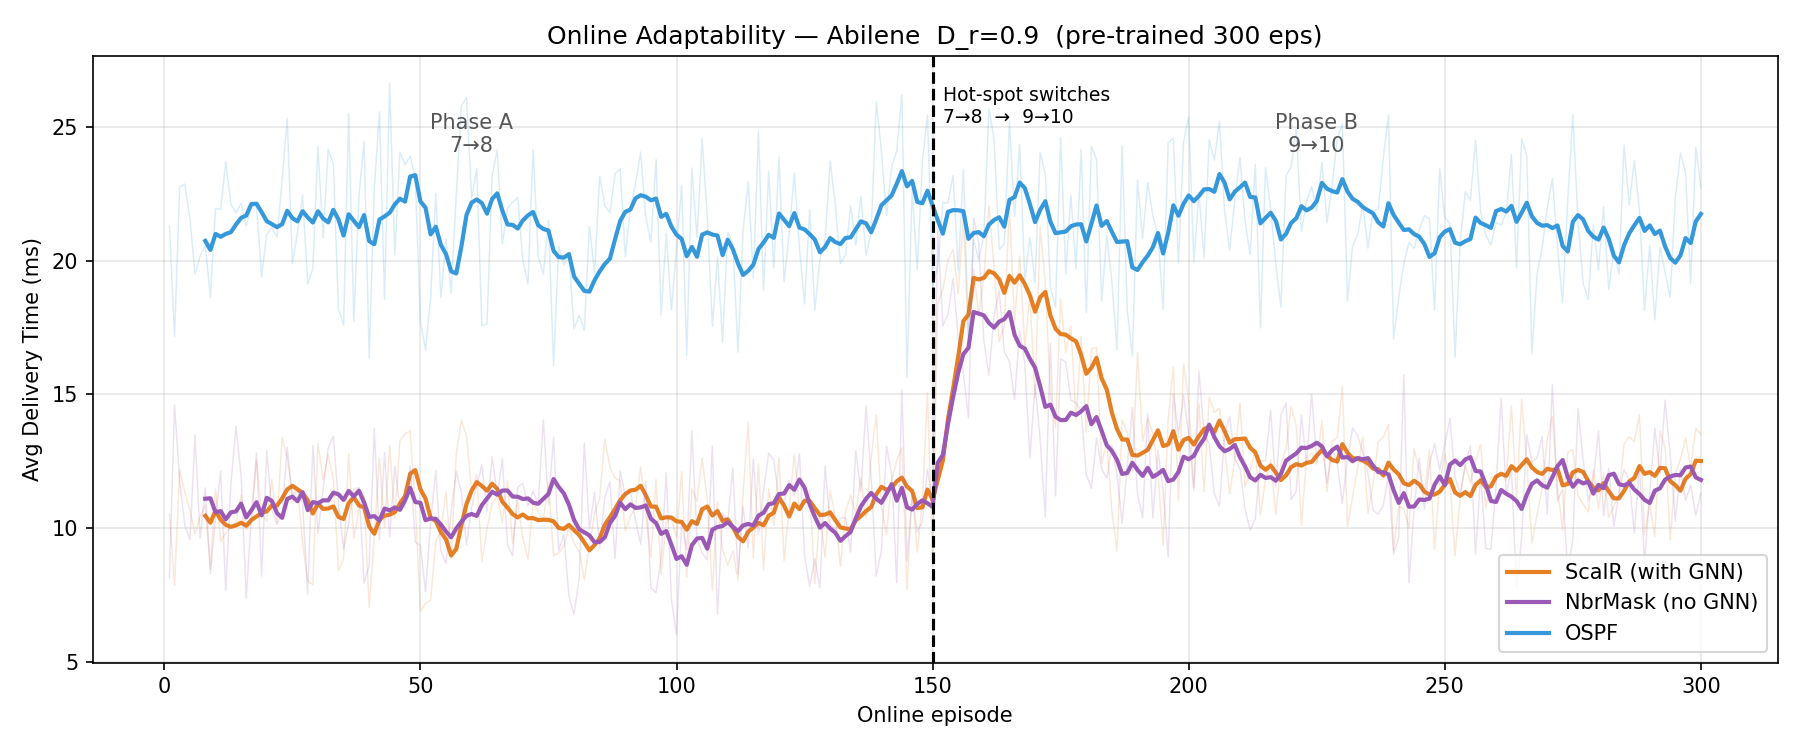
\includegraphics[width=\linewidth]{results/online_adaptability/online_adaptability.png}
\caption{Online adaptability on Abilene ($D_r = 0.9$). Both ScaIR (GNN)
and NbrMask (no GNN) are pre-trained for 300 episodes on hot-spot
7$\to$8. At online episode 151, the hot-spot shifts to 9$\to$10.
Both variants spike and re-converge at the same rate. OSPF remains
static at $\approx$21\,ms throughout.}
\label{fig:adapt}
\end{figure}

\subsection{Multi-hotspot: where does the model actually struggle?}

Given that ScaIR nearly saturates the single hot-spot problem in 300
episodes, we ask whether a genuinely harder scenario exists. We
construct a multi-hotspot scenario on Germany50 with four simultaneous
hot-spot pairs whose OSPF shortest paths all pass through the same
directed link corridor $25\!\to\!13\!\to\!49$, creating real
load-balancing competition. Each pair carries 15\% of total traffic
($D_r = 0.6$ in aggregate).

Under this scenario, OSPF reaches 12.8\,ms while an Oracle Greedy
baseline achieves 7.3\,ms. ScaIR trained for 800 episodes converges
to 7.6\,ms — still within 5\% of the Oracle, but requiring 800
episodes rather than 300. The training curve shows that by episode 300,
ScaIR has only just reached OSPF's level; the remaining convergence
from 12 to 7.6\,ms takes the full training budget. This confirms that
the model can learn harder coordination problems, but that the training
cost grows with problem complexity.

\section{Conclusions and Future Work}

Our investigation leads to a coherent picture of ScaIR's strengths and
limitations. Its gains over OSPF under congested traffic are genuine and
substantial — 40--80\% reductions in delivery time across four real
topologies — and they hold even on topologies with 50 nodes. However,
these gains stem from the multi-agent Q-network with UCB exploration
and local queue observations, not from the sub-GNN. The GNN's feature
vectors converge to a transformation of node identity labels; any fixed
encoding that provides the same identity information achieves equal or
better routing. ScaIR is, in practice, a distributed DQN with indexed
nodes where the GNN is an unnecessary and potentially harmful component.

The harmful aspect manifests under topology changes: when a new node is
inserted, its unknown identity corrupts the model's representations and
causes dramatic performance degradation. This is a direct consequence
of the one-hot origin of $\mathbf{V}_n$: the model generalises within
the set of identities it has seen, but not outside it.

An immediate direction for future work is to remove the one-hot
identifiers entirely from the initialisation and instead seed
$\mathbf{V}_n$ from observable structural properties — degree,
betweenness centrality, or shortest-path distance profiles — that
remain meaningful when the topology changes. We tested these initialisations
(Experiment 9, not reported here for space) and found no benefit within
300 episodes, suggesting the bottleneck is not the initialisation but
the entire identity-based parameterisation. A more promising direction
is to encode graph structure in a permutation-invariant manner from
the start, so that an unseen node with known connectivity can be
immediately placed in the model's representation space without retraining.

A second limitation is the simulation model itself. Our environment
models transmission as a single fixed delay per hop with no link
capacity constraints. Real networks have heterogeneous link speeds,
propagation delays, and finite buffers. Extending the environment to
include these would likely make congestion-aware routing more
beneficial and would test whether the GNN's structural information
becomes useful when the network physics are richer.

{\small
\bibliographystyle{ieee_fullname}
\begin{thebibliography}{9}

\bibitem{dijkstra1959}
E.~W. Dijkstra.
\newblock A note on two problems in connexion with graphs.
\newblock {\em Numerische Mathematik}, 1:269--271, 1959.

\bibitem{boyan1994}
J.~A. Boyan and M.~L. Littman.
\newblock Packet routing in dynamically changing networks: A reinforcement
  learning approach.
\newblock In {\em Advances in Neural Information Processing Systems (NIPS)},
  pages 671--678, 1994.

\bibitem{mukhutdinov2019}
D.~Mukhutdinov, A.~Filchenkov, A.~Shalyto, and V.~Vyatkin.
\newblock Multi-agent deep learning for simultaneous optimization for time and
  energy in distributed routing system.
\newblock {\em Future Generation Computer Systems}, 94:587--600, 2019.

\bibitem{you2020}
X.~You, X.~Li, Y.~Xu, H.~Feng, J.~Zhao, and H.~Yan.
\newblock Toward packet routing with fully distributed multiagent deep
  reinforcement learning.
\newblock {\em IEEE Transactions on Systems, Man, and Cybernetics},
  52(2):855--868, 2020.

\bibitem{bai2024}
J.~Bai, J.~Sun, Z.~Wang, X.~Zhao, A.~Wen, C.~Zhang, and J.~Zhang.
\newblock An adaptive intelligent routing algorithm based on deep reinforcement
  learning.
\newblock {\em Computer Communications}, 216:195--208, 2024.

\bibitem{rusek2020}
K.~Rusek, J.~Su{\'a}rez-Varela, P.~Almasan, P.~Barlet-Ros, and
  A.~Cabellos-Aparicio.
\newblock {RouteNet}: Leveraging graph neural networks for network modeling and
  optimization in {SDN}.
\newblock {\em IEEE Journal on Selected Areas in Communications},
  38(10):2260--2270, 2020.

\bibitem{scair2025}
J.~Zhang, J.~Guan, K.~Liu, Y.~Hu, A.~Shen, and Y.~Ma.
\newblock {ScaIR}: Scalable intelligent routing based on distributed graph
  reinforcement learning.
\newblock {\em Computer Networks}, 257:110915, 2025.

\bibitem{knight2011}
S.~Knight, H.~X. Nguyen, N.~Falkner, R.~Bowden, and M.~Roughan.
\newblock The internet topology zoo.
\newblock {\em IEEE Journal on Selected Areas in Communications},
  29(9):1765--1775, 2011.

\bibitem{sndlib}
S.~Orlowski, R.~Wess{\"a}ly, M.~Pi{\'o}ro, and A.~Tomaszewski.
\newblock {SNDlib} 1.0---survivable network design library.
\newblock {\em Networks}, 55(3):276--286, 2010.

\end{thebibliography}
}

\end{document}
